\begin{frame}
\frametitle{Baryon asymmetry in the Universe}
\framesubtitle{}

\vspace{-0.5cm}
 \begin{columns}
 \column{0.5\textwidth} 
    \begin{figure}
       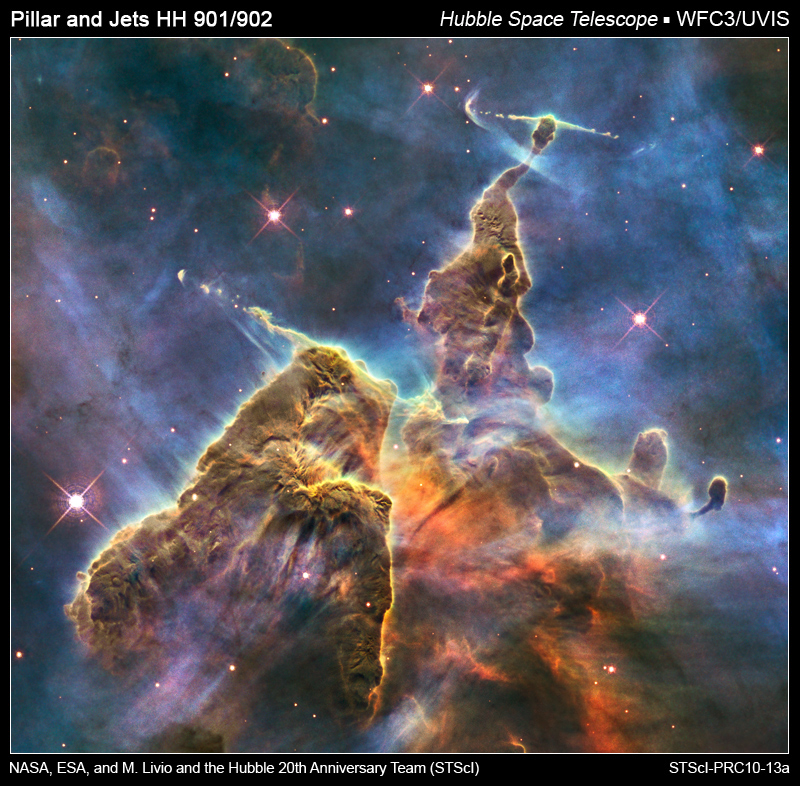
\includegraphics[width=0.6\textwidth]{carina}
    \end{figure}
 \column{0.45\textwidth} 
 \textbf{Carina Nebula:} Largest-seen star-birth regions in the galaxy
 \end{columns}

\begin{block}{\small Observation and expectation from Standard Cosmological Model (SCM):}
\begin{center}
\renewcommand*{\arraystretch}{1.3}\small
\begin{tabular}{l |l|l}
                       & $\eta = \displaystyle (n_b - n_{\bar{b}})/n_\gamma$ & \\\hline
 Observation              & $\left( 6.11^{+ 0.3}_{-0.2} \right) \times \num{e-10} $      &  Best Fit Cosmological Model\,\textcolor{PineGreen}{\cite{Bennett:2003bz}}\\
                       & $(5.53-6.76) \times \num{e-10}$ & WMAP\,\textcolor{PineGreen}{\cite{Barger:2003zg}} \\
 Expectation from SCM  & $\sim \num{e-18}$ & Bernreuther (2002)\,\textcolor{PineGreen}{\cite{Bernreuther:2002uj}}\\
\end{tabular}
\end{center}
\end{block}


\begin{alertblock}{}
 \begin{itemize}
 \item SCM gets it wrong by more than 8 orders of magnitude. 
\end{itemize}
\end{alertblock}

\end{frame}